\section{Data Handling for the Emitter}
\label{DataHandlingEmitter}

Figure \ref{fig:DHE}, on page \pageref{fig:DHE}, shows the data handling structure for the emitter satellite during nominal operating conditions. Nominal operating conditions refer to the state without any system failures. The rest of this section will contain some comments of the diagram is Figure \ref{fig:DHE}.

As can be seen the onboard computer is the most important part of the data handling subsystem. The term housekeeping data refers to all the data that indicate the spacecraft and its subsystems are in good health e.g. temperature, voltage, power, etc. It should also be noted that the S\&H arrow from the S-band antennae to the computer consists of science and housekeeping data from the receiver as well as  housekeeping data of the antennae. Furthermore the command going from the X-band phased array to the computer refers to commands sent up from the ground station, whereas all arrows pointing away from the computer refer to commands being send by the computer. One other exception is the command arrow pointing to the S-band antennae, as this includes commands to the antennae software and commands destined for the receiver satellites.

\begin{figure}
\centering
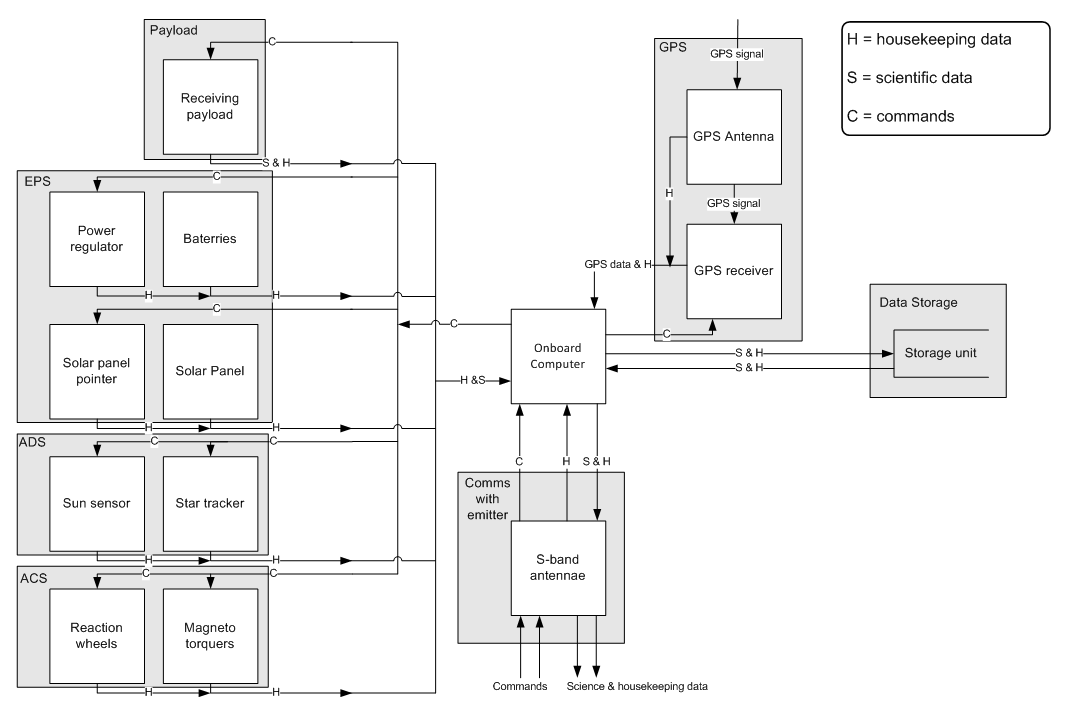
\includegraphics[width=1.0\textwidth, angle=90]{img/DHReceiver.png}
\caption{Figure showing the data handling structure for the emitter.}
\label{fig:DHE}
\end{figure}
